\begin{enumerate}[label=\thesection.\arabic*,ref=\thesection.\theenumi]
\numberwithin{equation}{enumi}
\numberwithin{figure}{enumi}
\numberwithin{table}{enumi}
\item In the Figure \ref{fig:9/9/2/1}, $ABCD$ is a parallelogram, $AE \perp DC$ and $CF \perp AD$. If $AB = 16 cm$, $AE = 8 cm$, and $CF = 10cm$, find $AD$.
	\begin{figure}[!h]
		\centering
 \includegraphics[width=\columnwidth]{chapters/9/9/2/1/figs/fig1.pdf}
		\caption{}
		\label{fig:9/9/2/1}
  	\end{figure}
\iffalse
\documentclass[journal,12pt,twocolumn]{IEEEtran}
\usepackage{setspace}
\usepackage{gensymb}
\usepackage{xcolor}
\usepackage{caption}
\singlespacing
\usepackage{siunitx}
\usepackage[cmex10]{amsmath}
\usepackage{mathtools}
\usepackage{hyperref}
\usepackage{amsthm}
\usepackage{mathrsfs}
\usepackage{txfonts}
\usepackage{stfloats}
\usepackage{cite}
\usepackage{cases}
\usepackage{subfig}
\usepackage{longtable}
\usepackage{multirow}
\usepackage{enumitem}
\usepackage{mathtools}
\usepackage{listings}
\usepackage{tikz}
\usetikzlibrary{shapes,arrows,positioning}
\usepackage{circuitikz}
\let\vec\mathbf
\DeclareMathOperator*{\Res}{Res}
\renewcommand\thesection{\arabic{section}}
\renewcommand\thesubsection{\thesection.\arabic{subsection}}
\renewcommand\thesubsubsection{\thesubsection.\arabic{subsubsection}}

\renewcommand\thesectiondis{\arabic{section}}
\renewcommand\thesubsectiondis{\thesectiondis.\arabic{subsection}}
\renewcommand\thesubsubsectiondis{\thesubsectiondis.\arabic{subsubsection}}
\hyphenation{op-tical net-works semi-conduc-tor}

\lstset{
language=Python,
frame=single, 
breaklines=true,
columns=fullflexible
}
\begin{document}
\theoremstyle{definition}
\newtheorem{theorem}{Theorem}[section]
\newtheorem{problem}{Problem}
\newtheorem{proposition}{Proposition}[section]
\newtheorem{lemma}{Lemma}[section]
\newtheorem{corollary}[theorem]{Corollary}
\newtheorem{example}{Example}[section]
\newtheorem{definition}{Definition}[section]
\newcommand{\BEQA}{\begin{eqnarray}}
\newcommand{\EEQA}{\end{eqnarray}}
\newcommand{\define}{\stackrel{\triangle}{=}}
\newenvironment{amatrix}[1]{%
  \left(\begin{array}{@{}*{#1}{c}|c@{}}
}{%
  \end{array}\right)
}
\newcommand{\myvec}[1]{\ensuremath{\begin{pmatrix}#1\end{pmatrix}}}
\newcommand{\myaugvec}[2]{\ensuremath{\begin{amatrix}{#1}#2\end{amatrix}}}
\newcommand{\mydet}[1]{\ensuremath{\begin{vmatrix}#1\end{vmatrix}}}
\bibliographystyle{IEEEtran}
\providecommand{\nCr}[2]{\,^{#1}C_{#2}} % nCr
\providecommand{\nPr}[2]{\,^{#1}P_{#2}} % nPr
\providecommand{\mbf}{\mathbf}
\providecommand{\pr}[1]{\ensuremath{\Pr\left(#1\right)}}
\providecommand{\qfunc}[1]{\ensuremath{Q\left(#1\right)}}
\providecommand{\sbrak}[1]{\ensuremath{{}\left[#1\right]}}
\providecommand{\lsbrak}[1]{\ensuremath{{}\left[#1\right.}}
\providecommand{\rsbrak}[1]{\ensuremath{{}\left.#1\right]}}
\providecommand{\brak}[1]{\ensuremath{\left(#1\right)}}
\providecommand{\lbrak}[1]{\ensuremath{\left(#1\right.}}
\providecommand{\rbrak}[1]{\ensuremath{\left.#1\right)}}
\providecommand{\cbrak}[1]{\ensuremath{\left\{#1\right\}}}
\providecommand{\lcbrak}[1]{\ensuremath{\left\{#1\right.}}
\providecommand{\rcbrak}[1]{\ensuremath{\left.#1\right\}}}
\theoremstyle{remark}
\newtheorem{rem}{Remark}
\newcommand{\sgn}{\mathop{\mathrm{sgn}}}
\newcommand{\rect}{\mathop{\mathrm{rect}}}
\newcommand{\sinc}{\mathop{\mathrm{sinc}}}
\providecommand{\abs}[1]{\left\vert#1\right\vert}
\providecommand{\res}[1]{\Res\displaylimits_{#1}} 
\providecommand{\norm}[1]{\left\Vert#1\right\Vert}
\providecommand{\mtx}[1]{\mathbf{#1}}
\providecommand{\mean}[1]{E\left[ #1 \right]}
\providecommand{\fourier}{\overset{\mathcal{F}}{ \rightleftharpoons}}
\providecommand{\ztrans}{\overset{\mathcal{Z}}{ \rightleftharpoons}}
\providecommand{\system}[1]{\overset{\mathcal{#1}}{ \longleftrightarrow}}
\newcommand{\solution}{\noindent \textbf{Solution: }}
\providecommand{\dec}[2]{\ensuremath{\overset{#1}{\underset{#2}{\gtrless}}}}
\let\StandardTheFigure\thefigure
\def\putbox#1#2#3{\makebox[0in][l]{\makebox[#1][l]{}\raisebox{\baselineskip}[0in][0in]{\raisebox{#2}[0in][0in]{#3}}}}
     \def\rightbox#1{\makebox[0in][r]{#1}}
     \def\centbox#1{\makebox[0in]{#1}}
     \def\topbox#1{\raisebox{-\baselineskip}[0in][0in]{#1}}
     \def\midbox#1{\raisebox{-0.5\baselineskip}[0in][0in]{#1}}

\vspace{3cm}
\title{Line Assignment}
\author{Gautam Singh}
\maketitle
\bigskip

\begin{abstract}
    This document contains the solution to Question 24 of Exercise 4 
    in Chapter 10 of the class 11 NCERT textbook.
\end{abstract}

\begin{enumerate}
\fi
		We first find the coordinates of the intersection of \eqref{eq:chapters/11/10/4/24/L1}
    and \eqref{eq:chapters/11/10/4/24/L2}. Using the augmented matrix and row reduction methods,
    \begin{align}
        \myaugvec{2}{2&-3&-4\\3&4&5} &\xleftrightarrow[]{R_2\rightarrow2R_2-3R_1} 
        \myaugvec{2}{2&-3&-4\\0&17&22} \\
                      &\xleftrightarrow[]{R_1\rightarrow17R_1+3R_2} \myaugvec{2}{17&0&-1\\0&17&22} \\
                      &\xleftrightarrow[]{\substack{R_1\rightarrow\frac{R_1}{17}\\R_2\rightarrow\frac{R_2}{17}}} \myaugvec{2}{1&0&-\frac{1}{17}\\0&1&\frac{22}{17}}
        \label{eq:chapters/11/10/4/24/intersect}
    \end{align}
    the intersection of the lines is
    \begin{align}
        \vec{A} = \frac{1}{17}\myvec{-1\\22}
    \end{align}
    Clearly, the man should follow the path perpendicular to \eqref{eq:chapters/11/10/4/24/L3} from
    $\vec{A}$ to reach it in the shortest time. The normal vector 
    of \eqref{eq:chapters/11/10/4/24/L3} is 
    \begin{align}
        \vec{m} = \myvec{6\\-7}
        \label{eq:chapters/11/10/4/24/L3-norm}
    \end{align}
    which is consequently the direction vector of the required line. Therefore, 
    the required normal vector is given by
    \begin{align}
        \vec{n} = \myvec{7\\6}
        \label{eq:chapters/11/10/4/24/L4-norm}
    \end{align}
    and hence, the equation of the line is
   \begin{align}
        \vec{n}^\top\vec{x} &= \vec{n}^\top\vec{A} \\
        \implies \myvec{7&6}\vec{x} &= \frac{1}{17}\myvec{7&6}\myvec{-1\\22} = \frac{125}{17}
        \label{eq:chapters/11/10/4/24/L4}
    \end{align}
		See Fig. \ref{fig:chapters/11/10/4/24/crossing}. In this figure $\vec{F}$ represents 
    the foot of the prependicular drawn from $\vec{A}$ onto \eqref{eq:chapters/11/10/4/24/L3}.

\item For a given Parallelogram $ABCD$, show that for any
point $\vec{P}$ inside the parallelogram,
\begin{enumerate}
	\item $Ar(APD)+Ar(PBC) = \frac{1}{2}Ar(ABCD)$
	\item $Ar(APD)+Ar(PBC) = Ar(APB)+Ar(PCD)$
\end{enumerate}
\iffalse
\documentclass[journal,12pt,twocolumn]{IEEEtran}
\usepackage{setspace}
\usepackage{gensymb}
\usepackage{xcolor}
\usepackage{caption}
\singlespacing
\usepackage{siunitx}
\usepackage[cmex10]{amsmath}
\usepackage{mathtools}
\usepackage{hyperref}
\usepackage{amsthm}
\usepackage{mathrsfs}
\usepackage{txfonts}
\usepackage{stfloats}
\usepackage{cite}
\usepackage{cases}
\usepackage{subfig}
\usepackage{longtable}
\usepackage{multirow}
\usepackage{enumitem}
\usepackage{mathtools}
\usepackage{listings}
\usepackage{tikz}
\usetikzlibrary{shapes,arrows,positioning}
\usepackage{circuitikz}
\let\vec\mathbf
\DeclareMathOperator*{\Res}{Res}
\renewcommand\thesection{\arabic{section}}
\renewcommand\thesubsection{\thesection.\arabic{subsection}}
\renewcommand\thesubsubsection{\thesubsection.\arabic{subsubsection}}

\renewcommand\thesectiondis{\arabic{section}}
\renewcommand\thesubsectiondis{\thesectiondis.\arabic{subsection}}
\renewcommand\thesubsubsectiondis{\thesubsectiondis.\arabic{subsubsection}}
\hyphenation{op-tical net-works semi-conduc-tor}

\lstset{
language=Python,
frame=single, 
breaklines=true,
columns=fullflexible
}
\begin{document}
\theoremstyle{definition}
\newtheorem{theorem}{Theorem}[section]
\newtheorem{problem}{Problem}
\newtheorem{proposition}{Proposition}[section]
\newtheorem{lemma}{Lemma}[section]
\newtheorem{corollary}[theorem]{Corollary}
\newtheorem{example}{Example}[section]
\newtheorem{definition}{Definition}[section]
\newcommand{\BEQA}{\begin{eqnarray}}
\newcommand{\EEQA}{\end{eqnarray}}
\newcommand{\define}{\stackrel{\triangle}{=}}
\newenvironment{amatrix}[1]{%
  \left(\begin{array}{@{}*{#1}{c}|c@{}}
}{%
  \end{array}\right)
}
\newcommand{\myvec}[1]{\ensuremath{\begin{pmatrix}#1\end{pmatrix}}}
\newcommand{\myaugvec}[2]{\ensuremath{\begin{amatrix}{#1}#2\end{amatrix}}}
\newcommand{\mydet}[1]{\ensuremath{\begin{vmatrix}#1\end{vmatrix}}}
\bibliographystyle{IEEEtran}
\providecommand{\nCr}[2]{\,^{#1}C_{#2}} % nCr
\providecommand{\nPr}[2]{\,^{#1}P_{#2}} % nPr
\providecommand{\mbf}{\mathbf}
\providecommand{\pr}[1]{\ensuremath{\Pr\left(#1\right)}}
\providecommand{\qfunc}[1]{\ensuremath{Q\left(#1\right)}}
\providecommand{\sbrak}[1]{\ensuremath{{}\left[#1\right]}}
\providecommand{\lsbrak}[1]{\ensuremath{{}\left[#1\right.}}
\providecommand{\rsbrak}[1]{\ensuremath{{}\left.#1\right]}}
\providecommand{\brak}[1]{\ensuremath{\left(#1\right)}}
\providecommand{\lbrak}[1]{\ensuremath{\left(#1\right.}}
\providecommand{\rbrak}[1]{\ensuremath{\left.#1\right)}}
\providecommand{\cbrak}[1]{\ensuremath{\left\{#1\right\}}}
\providecommand{\lcbrak}[1]{\ensuremath{\left\{#1\right.}}
\providecommand{\rcbrak}[1]{\ensuremath{\left.#1\right\}}}
\theoremstyle{remark}
\newtheorem{rem}{Remark}
\newcommand{\sgn}{\mathop{\mathrm{sgn}}}
\newcommand{\rect}{\mathop{\mathrm{rect}}}
\newcommand{\sinc}{\mathop{\mathrm{sinc}}}
\providecommand{\abs}[1]{\left\vert#1\right\vert}
\providecommand{\res}[1]{\Res\displaylimits_{#1}} 
\providecommand{\norm}[1]{\left\Vert#1\right\Vert}
\providecommand{\mtx}[1]{\mathbf{#1}}
\providecommand{\mean}[1]{E\left[ #1 \right]}
\providecommand{\fourier}{\overset{\mathcal{F}}{ \rightleftharpoons}}
\providecommand{\ztrans}{\overset{\mathcal{Z}}{ \rightleftharpoons}}
\providecommand{\system}[1]{\overset{\mathcal{#1}}{ \longleftrightarrow}}
\newcommand{\solution}{\noindent \textbf{Solution: }}
\providecommand{\dec}[2]{\ensuremath{\overset{#1}{\underset{#2}{\gtrless}}}}
\let\StandardTheFigure\thefigure
\def\putbox#1#2#3{\makebox[0in][l]{\makebox[#1][l]{}\raisebox{\baselineskip}[0in][0in]{\raisebox{#2}[0in][0in]{#3}}}}
     \def\rightbox#1{\makebox[0in][r]{#1}}
     \def\centbox#1{\makebox[0in]{#1}}
     \def\topbox#1{\raisebox{-\baselineskip}[0in][0in]{#1}}
     \def\midbox#1{\raisebox{-0.5\baselineskip}[0in][0in]{#1}}

\vspace{3cm}
\title{Line Assignment}
\author{Gautam Singh}
\maketitle
\bigskip

\begin{abstract}
    This document contains the solution to Question 24 of Exercise 4 
    in Chapter 10 of the class 11 NCERT textbook.
\end{abstract}

\begin{enumerate}
\fi
		We first find the coordinates of the intersection of \eqref{eq:chapters/11/10/4/24/L1}
    and \eqref{eq:chapters/11/10/4/24/L2}. Using the augmented matrix and row reduction methods,
    \begin{align}
        \myaugvec{2}{2&-3&-4\\3&4&5} &\xleftrightarrow[]{R_2\rightarrow2R_2-3R_1} 
        \myaugvec{2}{2&-3&-4\\0&17&22} \\
                      &\xleftrightarrow[]{R_1\rightarrow17R_1+3R_2} \myaugvec{2}{17&0&-1\\0&17&22} \\
                      &\xleftrightarrow[]{\substack{R_1\rightarrow\frac{R_1}{17}\\R_2\rightarrow\frac{R_2}{17}}} \myaugvec{2}{1&0&-\frac{1}{17}\\0&1&\frac{22}{17}}
        \label{eq:chapters/11/10/4/24/intersect}
    \end{align}
    the intersection of the lines is
    \begin{align}
        \vec{A} = \frac{1}{17}\myvec{-1\\22}
    \end{align}
    Clearly, the man should follow the path perpendicular to \eqref{eq:chapters/11/10/4/24/L3} from
    $\vec{A}$ to reach it in the shortest time. The normal vector 
    of \eqref{eq:chapters/11/10/4/24/L3} is 
    \begin{align}
        \vec{m} = \myvec{6\\-7}
        \label{eq:chapters/11/10/4/24/L3-norm}
    \end{align}
    which is consequently the direction vector of the required line. Therefore, 
    the required normal vector is given by
    \begin{align}
        \vec{n} = \myvec{7\\6}
        \label{eq:chapters/11/10/4/24/L4-norm}
    \end{align}
    and hence, the equation of the line is
   \begin{align}
        \vec{n}^\top\vec{x} &= \vec{n}^\top\vec{A} \\
        \implies \myvec{7&6}\vec{x} &= \frac{1}{17}\myvec{7&6}\myvec{-1\\22} = \frac{125}{17}
        \label{eq:chapters/11/10/4/24/L4}
    \end{align}
		See Fig. \ref{fig:chapters/11/10/4/24/crossing}. In this figure $\vec{F}$ represents 
    the foot of the prependicular drawn from $\vec{A}$ onto \eqref{eq:chapters/11/10/4/24/L3}.

\item In Fig.
		\ref{fig:9/9/2/5},
$PQRS$ and $ABRS$ are parallelograms
and $\vec{X}$ is any point on side $BR$. Show that  
\begin{enumerate}
    \item $ar (PQRS) = ar(ABRS)$
	    \label{prop:9/9/2/5}
    \item $ar(AXS) = \frac{1}{2} ar(PQRS)$
\end{enumerate}
	\begin{figure}[!h]
		\centering
 \includegraphics[width=\columnwidth]{chapters/9/9/2/5/figs/parallelogram1.pdf}
		\caption{}
		\label{fig:9/9/2/5}
  	\end{figure}
\iffalse
\documentclass[journal,12pt,twocolumn]{IEEEtran}
\usepackage{setspace}
\usepackage{gensymb}
\usepackage{xcolor}
\usepackage{caption}
\singlespacing
\usepackage{siunitx}
\usepackage[cmex10]{amsmath}
\usepackage{mathtools}
\usepackage{hyperref}
\usepackage{amsthm}
\usepackage{mathrsfs}
\usepackage{txfonts}
\usepackage{stfloats}
\usepackage{cite}
\usepackage{cases}
\usepackage{subfig}
\usepackage{longtable}
\usepackage{multirow}
\usepackage{enumitem}
\usepackage{mathtools}
\usepackage{listings}
\usepackage{tikz}
\usetikzlibrary{shapes,arrows,positioning}
\usepackage{circuitikz}
\let\vec\mathbf
\DeclareMathOperator*{\Res}{Res}
\renewcommand\thesection{\arabic{section}}
\renewcommand\thesubsection{\thesection.\arabic{subsection}}
\renewcommand\thesubsubsection{\thesubsection.\arabic{subsubsection}}

\renewcommand\thesectiondis{\arabic{section}}
\renewcommand\thesubsectiondis{\thesectiondis.\arabic{subsection}}
\renewcommand\thesubsubsectiondis{\thesubsectiondis.\arabic{subsubsection}}
\hyphenation{op-tical net-works semi-conduc-tor}

\lstset{
language=Python,
frame=single, 
breaklines=true,
columns=fullflexible
}
\begin{document}
\theoremstyle{definition}
\newtheorem{theorem}{Theorem}[section]
\newtheorem{problem}{Problem}
\newtheorem{proposition}{Proposition}[section]
\newtheorem{lemma}{Lemma}[section]
\newtheorem{corollary}[theorem]{Corollary}
\newtheorem{example}{Example}[section]
\newtheorem{definition}{Definition}[section]
\newcommand{\BEQA}{\begin{eqnarray}}
\newcommand{\EEQA}{\end{eqnarray}}
\newcommand{\define}{\stackrel{\triangle}{=}}
\newenvironment{amatrix}[1]{%
  \left(\begin{array}{@{}*{#1}{c}|c@{}}
}{%
  \end{array}\right)
}
\newcommand{\myvec}[1]{\ensuremath{\begin{pmatrix}#1\end{pmatrix}}}
\newcommand{\myaugvec}[2]{\ensuremath{\begin{amatrix}{#1}#2\end{amatrix}}}
\newcommand{\mydet}[1]{\ensuremath{\begin{vmatrix}#1\end{vmatrix}}}
\bibliographystyle{IEEEtran}
\providecommand{\nCr}[2]{\,^{#1}C_{#2}} % nCr
\providecommand{\nPr}[2]{\,^{#1}P_{#2}} % nPr
\providecommand{\mbf}{\mathbf}
\providecommand{\pr}[1]{\ensuremath{\Pr\left(#1\right)}}
\providecommand{\qfunc}[1]{\ensuremath{Q\left(#1\right)}}
\providecommand{\sbrak}[1]{\ensuremath{{}\left[#1\right]}}
\providecommand{\lsbrak}[1]{\ensuremath{{}\left[#1\right.}}
\providecommand{\rsbrak}[1]{\ensuremath{{}\left.#1\right]}}
\providecommand{\brak}[1]{\ensuremath{\left(#1\right)}}
\providecommand{\lbrak}[1]{\ensuremath{\left(#1\right.}}
\providecommand{\rbrak}[1]{\ensuremath{\left.#1\right)}}
\providecommand{\cbrak}[1]{\ensuremath{\left\{#1\right\}}}
\providecommand{\lcbrak}[1]{\ensuremath{\left\{#1\right.}}
\providecommand{\rcbrak}[1]{\ensuremath{\left.#1\right\}}}
\theoremstyle{remark}
\newtheorem{rem}{Remark}
\newcommand{\sgn}{\mathop{\mathrm{sgn}}}
\newcommand{\rect}{\mathop{\mathrm{rect}}}
\newcommand{\sinc}{\mathop{\mathrm{sinc}}}
\providecommand{\abs}[1]{\left\vert#1\right\vert}
\providecommand{\res}[1]{\Res\displaylimits_{#1}} 
\providecommand{\norm}[1]{\left\Vert#1\right\Vert}
\providecommand{\mtx}[1]{\mathbf{#1}}
\providecommand{\mean}[1]{E\left[ #1 \right]}
\providecommand{\fourier}{\overset{\mathcal{F}}{ \rightleftharpoons}}
\providecommand{\ztrans}{\overset{\mathcal{Z}}{ \rightleftharpoons}}
\providecommand{\system}[1]{\overset{\mathcal{#1}}{ \longleftrightarrow}}
\newcommand{\solution}{\noindent \textbf{Solution: }}
\providecommand{\dec}[2]{\ensuremath{\overset{#1}{\underset{#2}{\gtrless}}}}
\let\StandardTheFigure\thefigure
\def\putbox#1#2#3{\makebox[0in][l]{\makebox[#1][l]{}\raisebox{\baselineskip}[0in][0in]{\raisebox{#2}[0in][0in]{#3}}}}
     \def\rightbox#1{\makebox[0in][r]{#1}}
     \def\centbox#1{\makebox[0in]{#1}}
     \def\topbox#1{\raisebox{-\baselineskip}[0in][0in]{#1}}
     \def\midbox#1{\raisebox{-0.5\baselineskip}[0in][0in]{#1}}

\vspace{3cm}
\title{Line Assignment}
\author{Gautam Singh}
\maketitle
\bigskip

\begin{abstract}
    This document contains the solution to Question 24 of Exercise 4 
    in Chapter 10 of the class 11 NCERT textbook.
\end{abstract}

\begin{enumerate}
\fi
		We first find the coordinates of the intersection of \eqref{eq:chapters/11/10/4/24/L1}
    and \eqref{eq:chapters/11/10/4/24/L2}. Using the augmented matrix and row reduction methods,
    \begin{align}
        \myaugvec{2}{2&-3&-4\\3&4&5} &\xleftrightarrow[]{R_2\rightarrow2R_2-3R_1} 
        \myaugvec{2}{2&-3&-4\\0&17&22} \\
                      &\xleftrightarrow[]{R_1\rightarrow17R_1+3R_2} \myaugvec{2}{17&0&-1\\0&17&22} \\
                      &\xleftrightarrow[]{\substack{R_1\rightarrow\frac{R_1}{17}\\R_2\rightarrow\frac{R_2}{17}}} \myaugvec{2}{1&0&-\frac{1}{17}\\0&1&\frac{22}{17}}
        \label{eq:chapters/11/10/4/24/intersect}
    \end{align}
    the intersection of the lines is
    \begin{align}
        \vec{A} = \frac{1}{17}\myvec{-1\\22}
    \end{align}
    Clearly, the man should follow the path perpendicular to \eqref{eq:chapters/11/10/4/24/L3} from
    $\vec{A}$ to reach it in the shortest time. The normal vector 
    of \eqref{eq:chapters/11/10/4/24/L3} is 
    \begin{align}
        \vec{m} = \myvec{6\\-7}
        \label{eq:chapters/11/10/4/24/L3-norm}
    \end{align}
    which is consequently the direction vector of the required line. Therefore, 
    the required normal vector is given by
    \begin{align}
        \vec{n} = \myvec{7\\6}
        \label{eq:chapters/11/10/4/24/L4-norm}
    \end{align}
    and hence, the equation of the line is
   \begin{align}
        \vec{n}^\top\vec{x} &= \vec{n}^\top\vec{A} \\
        \implies \myvec{7&6}\vec{x} &= \frac{1}{17}\myvec{7&6}\myvec{-1\\22} = \frac{125}{17}
        \label{eq:chapters/11/10/4/24/L4}
    \end{align}
		See Fig. \ref{fig:chapters/11/10/4/24/crossing}. In this figure $\vec{F}$ represents 
    the foot of the prependicular drawn from $\vec{A}$ onto \eqref{eq:chapters/11/10/4/24/L3}.

%	
\item In quadrilateral $CBAD$,$CA = AD$ and $BA$ bisect $\angle{A}$ shown in figure \tabref{fig:chapters/9/7/1/1/Fig1}. Show that $\triangle{CAB} \cong \triangle{DAB}$. What can you say about $BC$ and $BD$? \\
	\solution
%\documentclass[12pt]{article}
%\usepackage[none]{hyphenat}
%\usepackage{amsmath}
%\usepackage{float}
%\usepackage{amssymb}
%\usepackage{graphicx}
%\usepackage{atbegshi}
%\AtBeginDocument{\AtBeginShipoutNext{\AtBeginShipoutDiscard}}
%\newcommand{\solution}{\noindent \textbf{Solution: }}
%\providecommand{\brak}[1]{\ensuremath{\left(#1\right)}}
%\newcommand{\myvec}[1]{\ensuremath{\begin{pmatrix}#1\end{pmatrix}}}
%\let\vec\mathbf
%\begin{document}
%\graphicspath{{./Documents}{./figs}}
%\begin{center}
%  \title{\textbf{Linear Forms}}
%  \date{\vspace{-5ex}}
%  \maketitle
%\end{center}
%\setcounter{page}{1}
%\section*{11$ ^{th} $ Maths - Chapter 10}
%The following problem is question 15 from exercise 10.3:
%\begin{enumerate}
%\item The perpendicular from the origin to the line $y=mx+c$ meets it at the point $(-1,2)$. Find the values of m and c.
%\end{enumerate}
%\solution \\
Given ,\\
the line line equation is

\begin{align}
   y&=mx+c
 \label{eq:1}
 \end{align}
\begin{align}
  \vec{P}&=\myvec{-1\\ \\2}\\
 \vec{O} &=\myvec{0\\ \\ 0}
\end{align}
   Direction Vector from $\vec{O}$ to point $\vec{P}$ is given by
    \begin{align}
    \vec{O - P} =\myvec{1\\ \\ -2}
 \end{align}
 If the lines are perpendicular then,
 \begin{align}
   \vec{(O - P)}^{\top}\vec{m} &= 0\\
   \myvec{1 & -2}\myvec{1 \\ \\ m}&=0\\
   1 - 2m &= 0\\
   m &= \frac{1}{2}
\end{align}
By substituting the m value in \eqref{eq:1},  we get
 \begin{align}
 2 &=\frac{1}{2} (-1) + c \\
 c &=\frac{5}{2}  
\end{align}
therefore,  Values of m and c are $\frac{1}{2}$ and $\frac{5}{2}$ \\
%\begin{figure}[H]
 % \centering
  %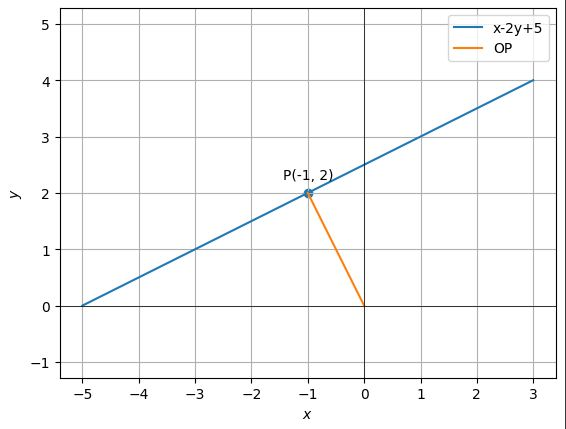
\includegraphics[width=\columnwidth]{figs/graph.jpg}
 % \caption{Graph}
 % \label{fig:pic}
%\end{figure}
%\end{document}

\item $ABCD$ is a quadrilateral in which $AD = BC$ and $\angle{DAB} = \angle{CBA}$ as shown in figure \ref{fig:chapters/9/7/1/2/Fig}. Prove that
\begin{enumerate}
\item $\triangle{ABD} \cong \triangle{BAC}$
  \item $BD = AC$
  \item $\angle{ABD} = \angle{BAC}$
\end{enumerate}
	\solution
%\documentclass[12pt]{article}
%\usepackage[none]{hyphenat}
%\usepackage{amsmath}
%\usepackage{float}
%\usepackage{amssymb}
%\usepackage{graphicx}
%\usepackage{atbegshi}
%\AtBeginDocument{\AtBeginShipoutNext{\AtBeginShipoutDiscard}}
%\newcommand{\solution}{\noindent \textbf{Solution: }}
%\providecommand{\brak}[1]{\ensuremath{\left(#1\right)}}
%\newcommand{\myvec}[1]{\ensuremath{\begin{pmatrix}#1\end{pmatrix}}}
%\let\vec\mathbf
%\begin{document}
%\graphicspath{{./Documents}{./figs}}
%\begin{center}
%  \title{\textbf{Linear Forms}}
%  \date{\vspace{-5ex}}
%  \maketitle
%\end{center}
%\setcounter{page}{1}
%\section*{11$ ^{th} $ Maths - Chapter 10}
%The following problem is question 15 from exercise 10.3:
%\begin{enumerate}
%\item The perpendicular from the origin to the line $y=mx+c$ meets it at the point $(-1,2)$. Find the values of m and c.
%\end{enumerate}
%\solution \\
Given ,\\
the line line equation is

\begin{align}
   y&=mx+c
 \label{eq:1}
 \end{align}
\begin{align}
  \vec{P}&=\myvec{-1\\ \\2}\\
 \vec{O} &=\myvec{0\\ \\ 0}
\end{align}
   Direction Vector from $\vec{O}$ to point $\vec{P}$ is given by
    \begin{align}
    \vec{O - P} =\myvec{1\\ \\ -2}
 \end{align}
 If the lines are perpendicular then,
 \begin{align}
   \vec{(O - P)}^{\top}\vec{m} &= 0\\
   \myvec{1 & -2}\myvec{1 \\ \\ m}&=0\\
   1 - 2m &= 0\\
   m &= \frac{1}{2}
\end{align}
By substituting the m value in \eqref{eq:1},  we get
 \begin{align}
 2 &=\frac{1}{2} (-1) + c \\
 c &=\frac{5}{2}  
\end{align}
therefore,  Values of m and c are $\frac{1}{2}$ and $\frac{5}{2}$ \\
%\begin{figure}[H]
 % \centering
  %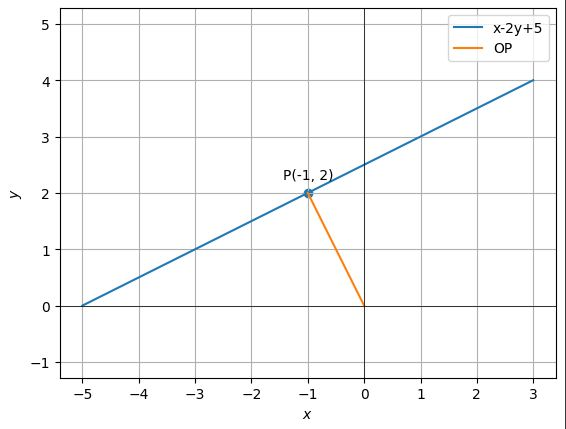
\includegraphics[width=\columnwidth]{figs/graph.jpg}
 % \caption{Graph}
 % \label{fig:pic}
%\end{figure}
%\end{document}

\item $AD$ and $BC$ are equal perpendiculars to a line segment $AB$. Show that $CD$ bisects $AB$.\\
	\solution
%\documentclass[12pt]{article}
%\usepackage[none]{hyphenat}
%\usepackage{amsmath}
%\usepackage{float}
%\usepackage{amssymb}
%\usepackage{graphicx}
%\usepackage{atbegshi}
%\AtBeginDocument{\AtBeginShipoutNext{\AtBeginShipoutDiscard}}
%\newcommand{\solution}{\noindent \textbf{Solution: }}
%\providecommand{\brak}[1]{\ensuremath{\left(#1\right)}}
%\newcommand{\myvec}[1]{\ensuremath{\begin{pmatrix}#1\end{pmatrix}}}
%\let\vec\mathbf
%\begin{document}
%\graphicspath{{./Documents}{./figs}}
%\begin{center}
%  \title{\textbf{Linear Forms}}
%  \date{\vspace{-5ex}}
%  \maketitle
%\end{center}
%\setcounter{page}{1}
%\section*{11$ ^{th} $ Maths - Chapter 10}
%The following problem is question 15 from exercise 10.3:
%\begin{enumerate}
%\item The perpendicular from the origin to the line $y=mx+c$ meets it at the point $(-1,2)$. Find the values of m and c.
%\end{enumerate}
%\solution \\
Given ,\\
the line line equation is

\begin{align}
   y&=mx+c
 \label{eq:1}
 \end{align}
\begin{align}
  \vec{P}&=\myvec{-1\\ \\2}\\
 \vec{O} &=\myvec{0\\ \\ 0}
\end{align}
   Direction Vector from $\vec{O}$ to point $\vec{P}$ is given by
    \begin{align}
    \vec{O - P} =\myvec{1\\ \\ -2}
 \end{align}
 If the lines are perpendicular then,
 \begin{align}
   \vec{(O - P)}^{\top}\vec{m} &= 0\\
   \myvec{1 & -2}\myvec{1 \\ \\ m}&=0\\
   1 - 2m &= 0\\
   m &= \frac{1}{2}
\end{align}
By substituting the m value in \eqref{eq:1},  we get
 \begin{align}
 2 &=\frac{1}{2} (-1) + c \\
 c &=\frac{5}{2}  
\end{align}
therefore,  Values of m and c are $\frac{1}{2}$ and $\frac{5}{2}$ \\
%\begin{figure}[H]
 % \centering
  %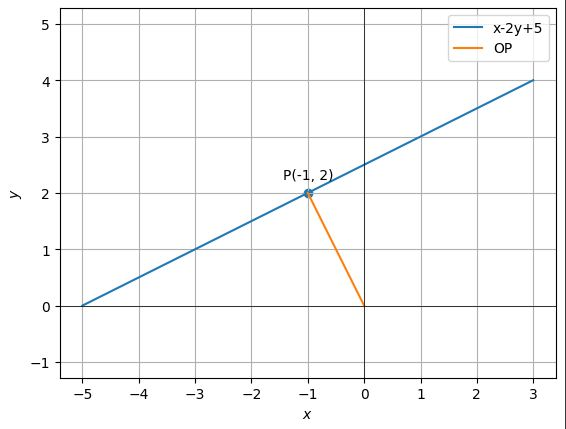
\includegraphics[width=\columnwidth]{figs/graph.jpg}
 % \caption{Graph}
 % \label{fig:pic}
%\end{figure}
%\end{document}

\item
$l$ and $m$ are two parallel lines intersected by another pair of parallel lines $p$ and $q (\figref{fig:9.7.1.4})$,show that $\triangle ABC \cong \triangle CDA$.

\textbf{Figure :}
\begin{figure}[H]
    \centering
	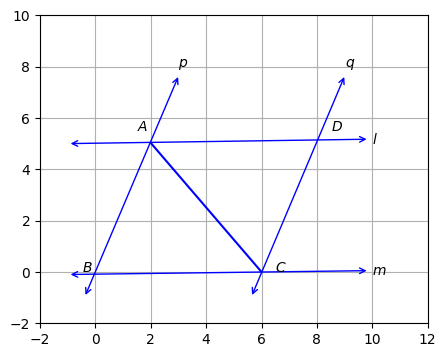
\includegraphics[width=\columnwidth]{chapters/9/7/1/4/fig/em1.png}
    \caption{Required parallelogram}
    \label{fig:9.7.1.4}
\end{figure}

\textbf{Solution :}
\begin{table}[H]
    \centering
      \begin{tabular}{|c|c|c|}
    \hline
        \textbf{Symbol} &\textbf{Description}&\textbf{Value}  \\
        \hline
        $\vec{B}$&Vertex at origin&$\vec{0}$\\
        \hline
        $a$ & Side of the parallelogram,$BC=DA$ & 6\\
        \hline
        $b$ & Side of the parallelogram,$AB=CD$& $\sqrt{29}$\\
        \hline
        $\theta$ & Angle of the parallelogram, $\angle ABC$& $\sin^{-1}\brak{{\frac{5}{\sqrt{29}}}}$\\
        \hline
    \end{tabular}

    \caption{Table of input parameters}
    \label{tab:9.7.1.4.1}
\end{table}

\begin{table}[H]
    \centering
     \begin{tabular}{|c|c|c|}
    \hline
        \textbf{Symbol} &\textbf{Description}&\textbf{Value}  \\
        \hline
  $\vec{C}$&Vertex of parallelogram &$a\vec{e_1}$\\
        \hline
         $\vec{A}$&Vertex of parallelogram &$b\myvec{
             \cos{\theta}\\
             \sin{\theta}
         }$\\
        \hline
        $\vec{D}$&Vertex of parallelogram &$\vec{C+A}$\\
        \hline
    \end{tabular}


    \caption{Table of output parameters}
    \label{tab:9.7.1.4.2}
\end{table}  
So,$\triangle ABC \cong \triangle CDA.\brak{by A-A-S}\brak{proved}$


\item Line $l$ is the bisector of an angle $\angle{A}$ and $B$ is a point on line $l$. $BP = BQ$ are perpendiculars from $B$ to the arms of $\angle{A}$. 
\begin{enumerate}
\item $\triangle{APB} \cong \triangle{AQB}$
\item $BP = BQ$ or $B$ is equidistant from the arms of $\angle{A}$
\end{enumerate}

\textbf{Construction}\\
The input parameters for the construction are shown in Table 
\begin{figure}[H]
    \begin{center}
     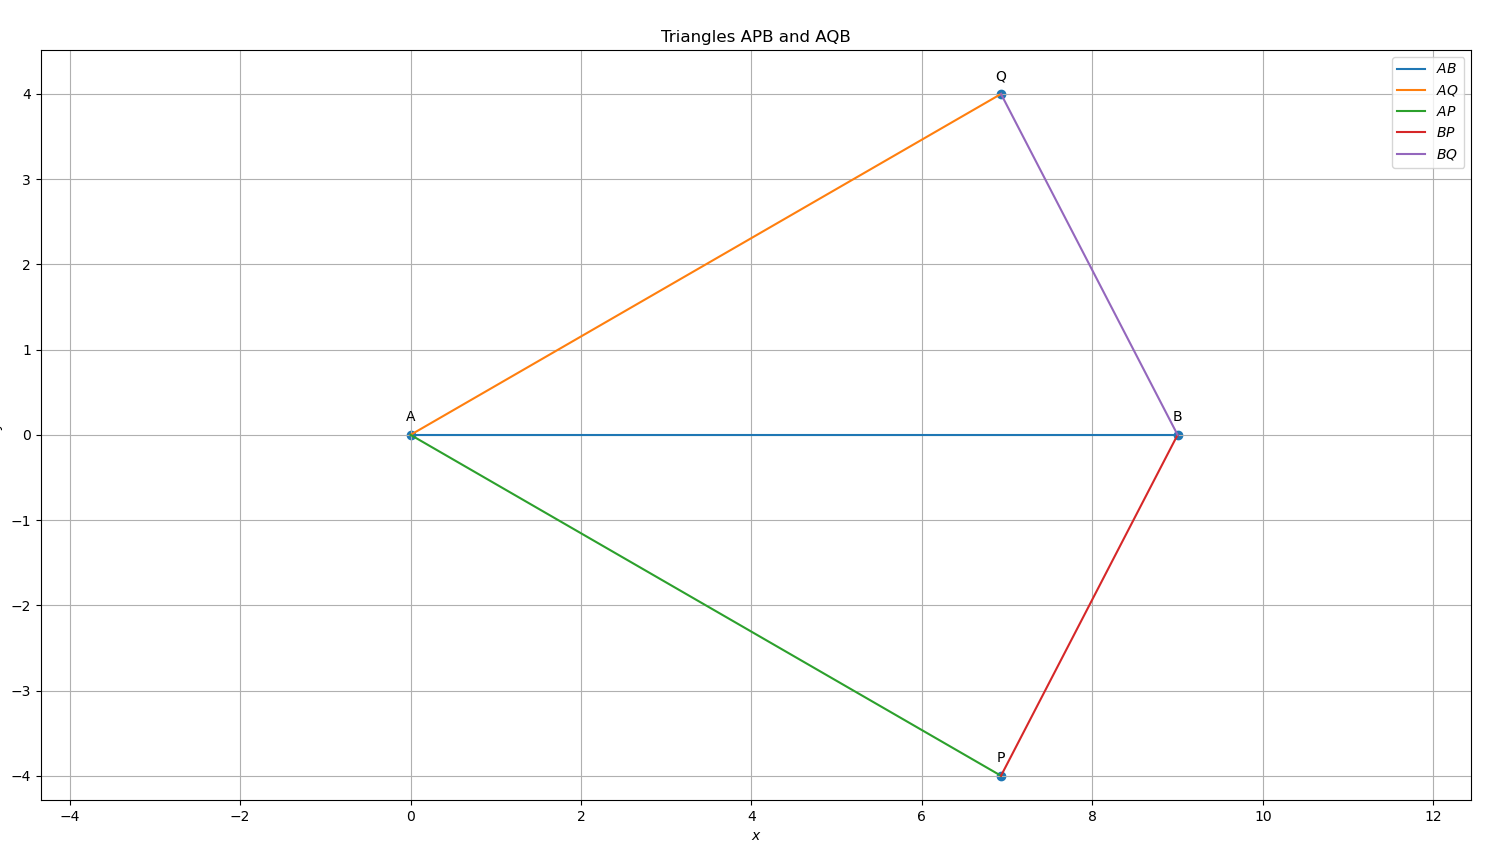
\includegraphics[width=\columnwidth]{chapters/9/7/1/5/figs/tri.png}
    \caption{figure}
    \label{fig:chapters/9/7/1/5/figs/tri.png}   
    \end{center}
\end{figure}

\begin{table}[h]
	  \centering
	  \begin{tabular}{|c|c|p{5cm}|}
\hline
\textbf{Symbol} & \textbf{Value} & \textbf{Description} \\
\hline
$\theta$ & $30\degree$ & $\angle{BAP} = \angle{BAQ}$ \\
\hline
$a$ & $9$ & $AB$ \\
\hline
$c$ & $8$ & $AQ$ \\
\hline
$\vec{e}_1$ & $\myvec{1\\0}$ & Basis vector \\
\hline
\end{tabular}

	  \caption{Parameters}
	  \label{Table}
\end{table}

Let $\vec{A} = \myvec{0\\0}$, $\vec{B} = a\vec{e_1}$, $\vec{Q} = \myvec{c\cos\theta\\c\sin\theta}$, and $\vec{P} = \myvec{c\cos\theta\\-c\sin\theta}$.


\end{enumerate}
